\section{Hybrid Prefetcher}
\label{sec:prefetcher}
% This section explains your proposed solution in full detail.
% It needs to strike a fine balance between unnecessary implementation
% details and a level of abstraction that is too high.
% The goal is to give enough detail such that the audience of
% your paper is able to reimplement your scheme, but not more.
% Informative figures and examples are a very powerful tool for
% conveying necessary information to your audience, and are
% often worth more than a thousand words.

The final prefetcher implemented during this project keeps a history of the
previous memory requests issued and uses three different algorithms in a
prioritized order to determine which addresses to prefetch.
An overview can be found in Figure \ref{fig:prefetcher}.

\begin{figure*}[h]
	\centering
	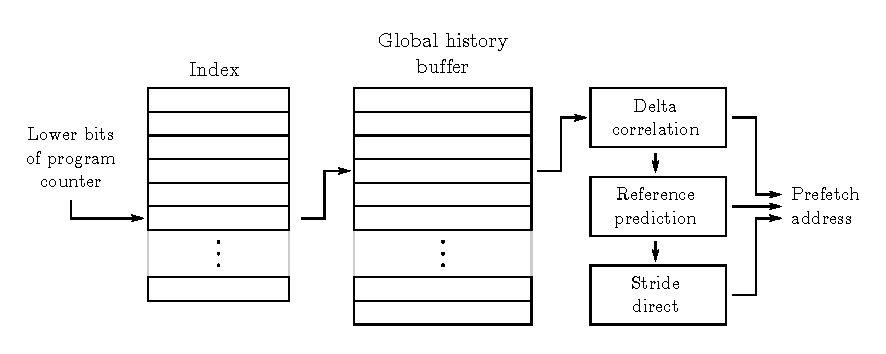
\includegraphics{images/prefetcher.pdf}
	\caption{
		Basic structure and data flow in prefetcher. The lower bits of the
		program counter at the load instruction is used to look up the first
		entry of a history chain in the global history buffer. Next, the history
		is used to determine which addresses to prefetch using one of the
		algorithms on the right.
	}
	\label{fig:prefetcher}
\end{figure*}

The history tracking is implemented using a global history buffer and an index.
Given an instruction address, the lower bits can be used to look up an entry in
the global history buffer through the index.
This entry is the first in a doubly linked list of memory addresses accessed by
instructions with matching lower bits in their addresses.

On a memory request, the index and global history buffer is updated and the
linked list of addresses is used to calculate a history of deltas, the
differences between consecutive memory addresses in the list.
This list is passed on to the algorithms used to determine which addresses to
prefetch.

First in line is the delta correlation algorithm.
It searches the history for the two most recent deltas.
If found, we assume to have found a loop of deltas and issue prefetches for the
addresses following the current with the deltas from the history.
In the cases where the degree is higher than the length of the matching history,
the process is repeated from the last memory address prefetched until enough
prefetches have been issued.
This strategy fails to produce prefetches when

\begin{enumerate}
	\item the history contains less than 3 entries for the given program
		counter or
	\item the two most recent deltas do not appear anywhere earlier in the
		history.
\end{enumerate}

Should the delta correlation fail to produce prefetches, the delta history is
handed on to an algorithm inspired by the reference prediction table.
The prefetches are issued using the most recent delta in the history if the two
last entries are equal.
In this case, the same delta is simply added to the memory address requested
several times to produce all prefetch addresses.

In the cases where the history contains one, and only one delta, the prefetcher
uses this delta to issue prefetches as for the previous algorithm.
This is equivalent to what a stride directed prefetcher would do.

It is important to note that both the index and the global history buffer is
limited in size. For the history buffer, this is handled by overwriting the
oldest entry. For the index, only the lower bits of the instruction address is
used, thus we may experience collisions.

%TODO: Can we assume there to be a low number of collisions based on the results
%      from associative caches in Computer Architecture: A Quantitative Approach?
